\documentclass{beamer}

\usepackage[utf8]{inputenc}
\usepackage{default}
\usepackage{latexsym,amsfonts,graphicx,amssymb}
\usepackage{amsfonts,amsthm,amsmath,amssymb,array,bm}
\usepackage{color}
% \usepackage{anysize}
\usepackage{hyperref}
\usepackage{chngcntr}
\usetheme{Madrid}
\usecolortheme{beaver}

\newtheorem{thm}{Theorem}[section]
\newtheorem{lem}{Lemma}[section]
\newtheorem{cor}{Corollary}[section]
\newtheorem{rem}{Note}[section]
\newtheorem{expls}{Example}[section]
\newtheorem{conj}{Conjecture}[section]

\DeclareMathOperator*{\argmin}{argmin}
\DeclareMathOperator*{\argmax}{argmax}

\mode<presentation>{}
\setbeamercolor{alerted text}{fg=blue!75}
\setbeamerfont{alerted text}{series=\bfseries}
% colored alerts
\newcommand{\alertg}[1]{\textcolor{black!40!green!75}{\bf #1}}
\newcommand{\alerto}[1]{\textcolor{orange!75}{\bf #1}}
\newcommand{\alertv}[1]{\textcolor{violet!75}{\bf #1}}
% colored boxes
\newcommand{\boxgreen}[1]{\fcolorbox{white}{black!25!green!25}{#1}}
\newcommand{\boxblue}[1]{\fcolorbox{white}{blue!25}{#1}}
\newcommand{\boxorange}[1]{\fcolorbox{white}{orange!25}{#1}}
\newcommand{\boxviolet}[1]{\fcolorbox{white}{violet!25}{#1}}
\newcommand{\boxinvis}[1]{\fcolorbox{white}{black!0}{#1}}

\title[Project 5]{Project 5: Modelling the performance of the rechargeable Li-Ion batteries}
\author[]{Sebastian Dominguez,
\quad Raed Mara'Beh,
\quad Alamgir Hossain,\\
\quad Helena Ribera,
\quad Zhenhua Lin,
\quad Hatef Dastour,
\quad Samad Bhuiyan\\
\vspace{0.5cm} MENTOR: Brian Wetton, University of British Columbia\\
{\it Graduate MMIW 2016}}

\begin{document}
\begin{frame}
 \titlepage
%  \vspace{-2cm}
%  \begin{figure}[h!]
% \hspace{8cm}\includegraphics[scale=0.04]{../sfu-logo.png}
%  \end{figure}
\end{frame}

\begin{frame}
 %\section*{Outline}
 \frametitle{Outline}
 \tableofcontents
\end{frame}

\section{Introduction}
\begin{frame}
 \frametitle{Background}
{\Large
A lithium-ion battery ( Li-ion battery ) is a member of a family of rechargeable battery types in which lithium ions move from the negative electrode to the positive electrode during discharge and back when charging.}
%Lithium-ion batteries are increasingly used in many systems, such as portable e%lectronics
%, electric vehicles, space and aircraft power systems, and  stationary power storage.}

\vspace{1cm}

\centering
\includegraphics[width=5cm]{DSC_2680.jpg}
\quad \includegraphics[width=5cm]{swingcell.jpg}
\end{frame}

\begin{frame}
  \frametitle{Li-ion batteries}
Li-ion batteries have many feautures:
\begin{itemize}
\item High energy density.
\item Long stable power and long run time.
\item Ideal for notebook, PCs, boosters, portable devices, etc.
\end{itemize}\\

 Definitions:\\
 C-rate: designates the rate at which the battery capacity can be  consumed or filled.
 \[ \textrm{I =capacity x C-rate}\]
 EMF: Electromotive force, is the voltage developed by any source of electrical energy such as a battery.\\

\end{frame}

\begin{frame}
 \frametitle{Some Targets}
 \begin{itemize}
% \item How do we fit a model to investigate a  Battery Management System?
   %  \bigskip
 \item State of Charge (SOC) and Voltage or Current (or a relationship between them) algebraically determines the rate
   of change in the SOC.
   \item First target: empirical fit to this relationship. %(example: low voltage initial charging).
\item Equivalent circuit models or system Identification (black box
  fit).
 \end{itemize}
 
 \centering{\textcolor{red}{Scientific challenge:}  How do we fit a model for parallel and series cells to investigate the performance and failure statistics in parallel versus
series designs ?}
% Some prelimary results will be shown in the following: 
\end{frame}


%\begin{frame}{Battery management system}

%A battery management system (BMS) is any electronic system that manages a rechargeable battery (cell or battery pack), such as by protecting the battery from operating outside its Safe Operating Area, monitoring its state, calculating secondary data, reporting that data, controlling its environment, authenticating it and / or balancing it.


%\end{frame}
%\begin{frame}{Monitoring}
%\begin{itemize}
%\item Voltage: total voltage, voltages of individual cells, minimum and maximum cell voltage or
%\item  Temperature: average temperature, coolant intake temperature, coolant output temperature,
 %or temperatures of individual cells
%\item  State of charge (SoC) to indicate the charge level of the battery
%\item  Current: current in or out of the battery
%\end{itemize}

%\end{frame}

%\begin{frame}
% \frametitle{Targets}
% \begin{itemize}
%\item Investigate  Battery Management System 
%\item  Investigate performance and failure statistics in parallel versus
%series designs.
%\end{itemize}
%\end{frame}

%\begin{frame}
% From targets from Brian's presentation:
%\end{frame}


\section{Experimental data}
\begin{frame}
\frametitle{Primary Results: Charge Characteristics}
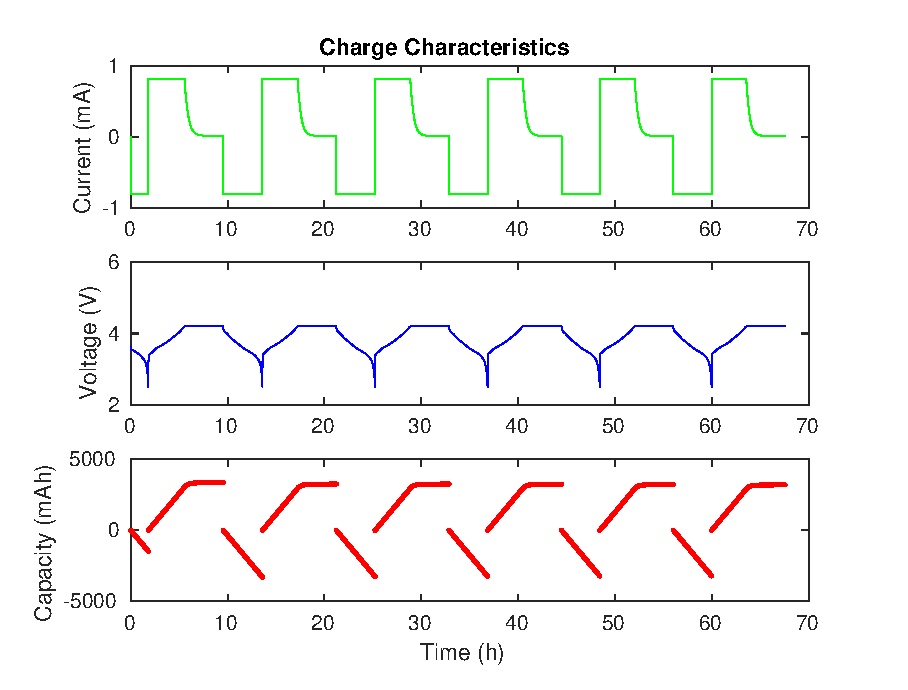
\includegraphics[width=6cm]{ChargeCharacteristicAllCycle-C.eps}
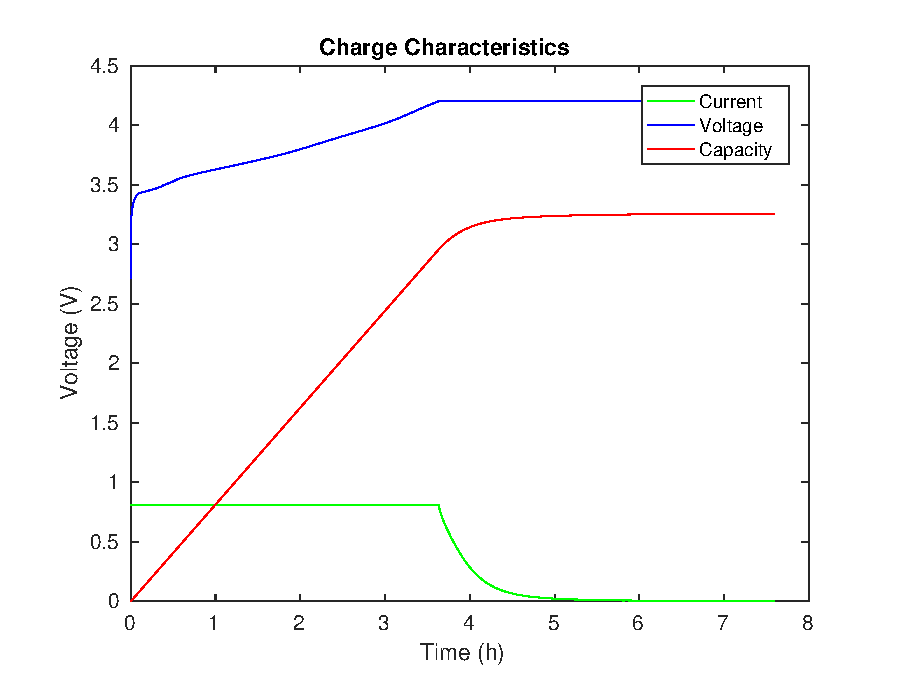
\includegraphics[width=6cm]{ChargeCharacteristicOneCycle-C.eps}
\end{frame}
%--------------------------------------------------------------

\begin{frame}
\frametitle{Primary Results: More Characteristics}
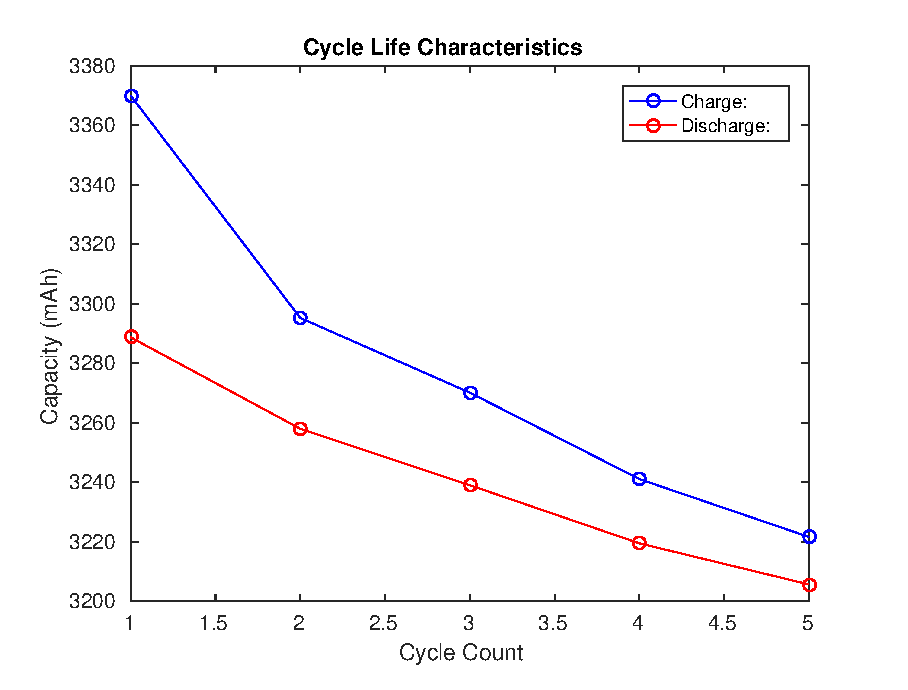
\includegraphics[width=6cm]{CycleLifeCharacteristics-C.eps}
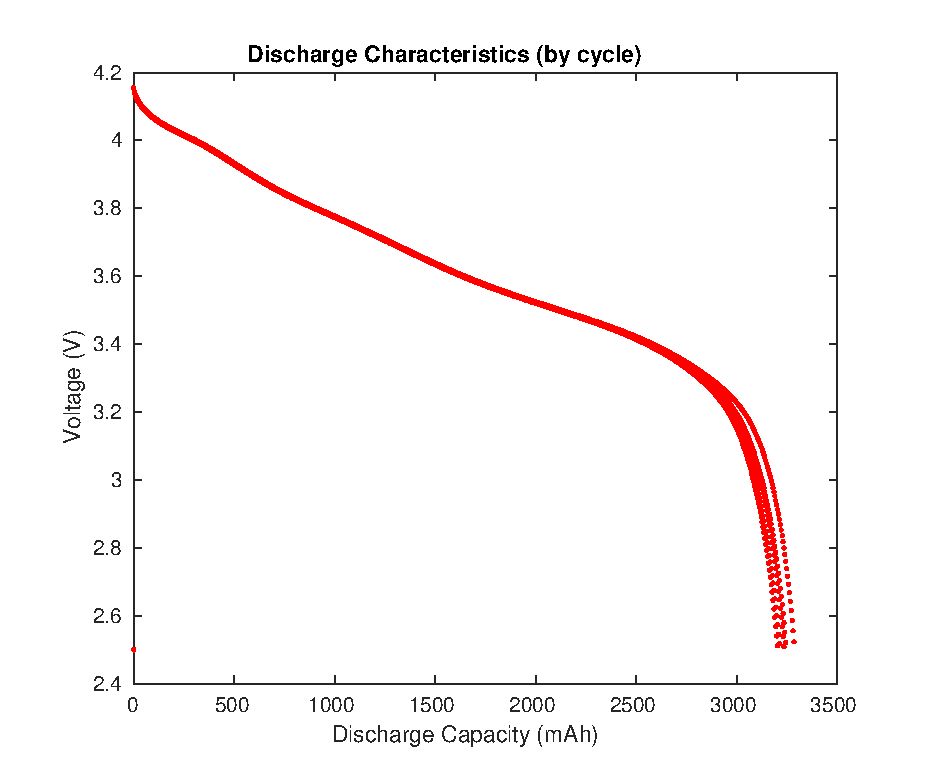
\includegraphics[width=6cm]{DischargeCharacteristics-C.eps}
\end{frame}
%----------------------------------------------------------------

%\begin{frame}
%\frametitle{Discharge Characteristics}
%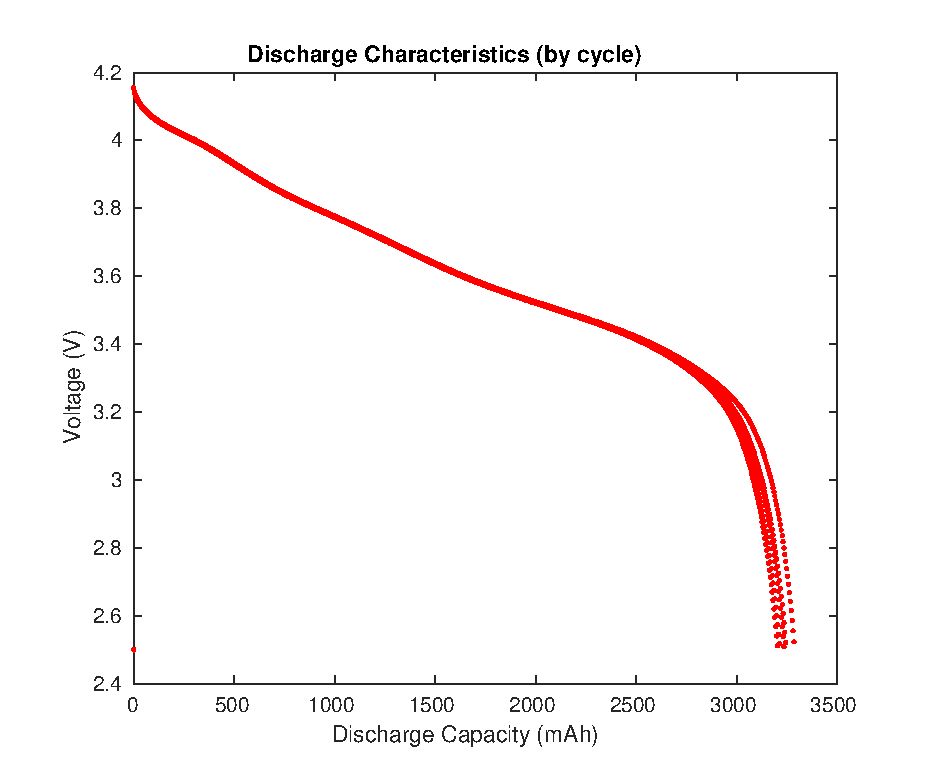
\includegraphics[width=6cm]{DischargeCharacteristics-C.eps}
%\end{frame}
%----------------------------------------------------------------

\begin{frame}
  \frametitle{Primary Results: EMF curves}
  \centering
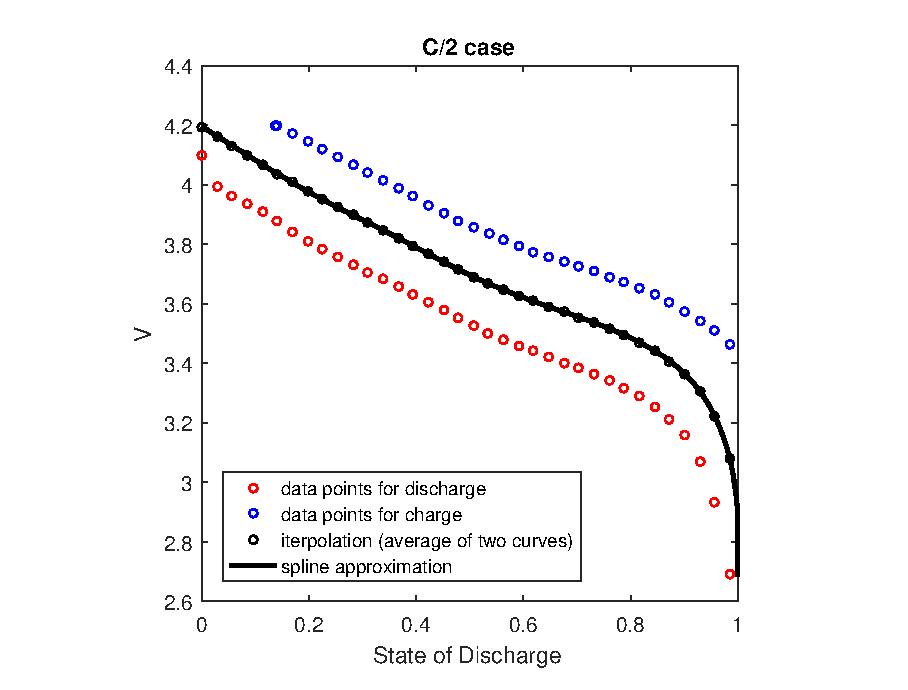
\includegraphics[width=5cm]{HRP_C2.eps}
~
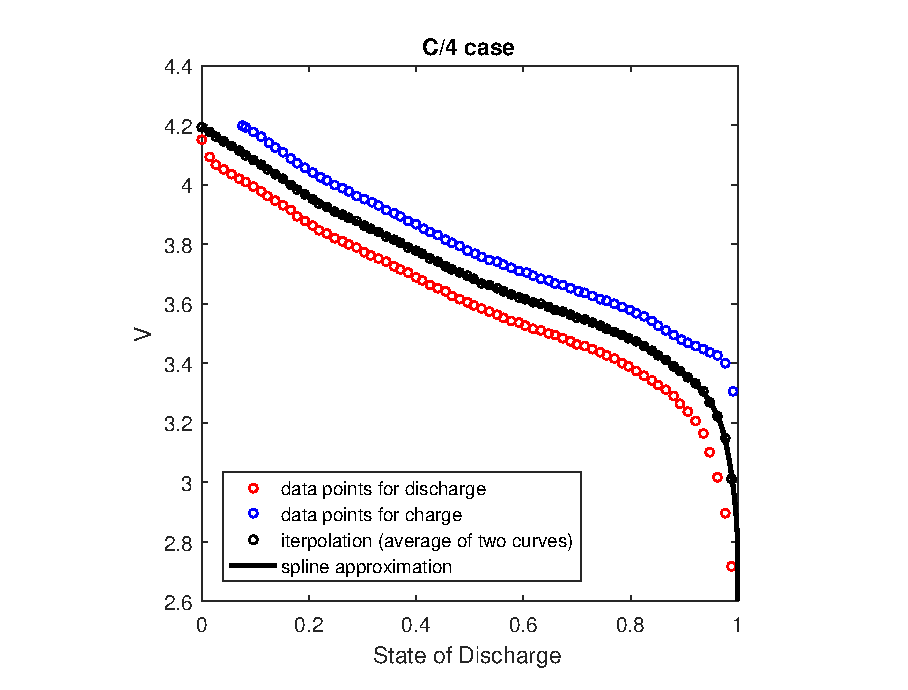
\includegraphics[width=5cm]{HRP_C4.eps}\\
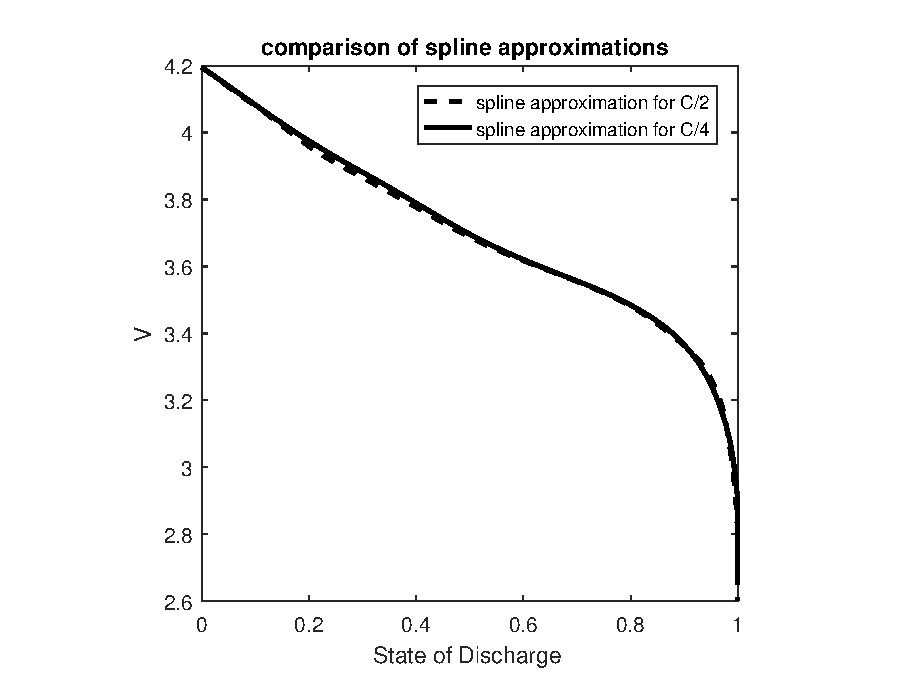
\includegraphics[width=5cm]{HRP_C2andC4_spline_comparison.eps}
\end{frame}
%----------------------------------------------------------------
\section{EMF and Model}
\begin{frame}
\frametitle{Mathematical Model}
\[ R_2 C \frac{d \mathcal{V}}{d t} + \mathcal{V} = R_2 C \frac{d E}{d t} - C R_1 R_2 \frac{d i}{d t} + E -(R_1 + R_2) i \]
\centering

\begin{minipage}{.5\textwidth}
\centering
\begin{itemize}
\item C - Capacitance (F)
\item $\mathcal{V}$ - Battery voltage (V).
  \item $E$ - Battery equilibrium potential (V)
  \item $R_1, R_2$ Resistance ($\Omega$)
  \item $i$ - Battery current (A).
\end{itemize}
      
\end{minipage}%
\begin{minipage}{0.5\textwidth}
\includegraphics[width=4cm]{circuit.png}\\
\centering
\caption{Equivalent circuit representation of lithium-ion cell.}
\end{minipage}
\end{frame}
%----------------------------------------------------------------
\section{Future work}
\begin{frame}
  \frametitle{Ongoing work}
\begin{itemize}
\item validation with expermiental data for constant resistance 
\item parallel and series cell model
  \item describe the model by the system of differential algebric equations 
\end{itemize}
\centerline{\includegraphics[width=5cm]{TheCircuit}}
\end{frame}


%\section{References}
% \vspace{2cm}
% \begin{thebibliography}{30}
% \bibitem{duran}
% {\sc M. G. Armentano and R. G. Dur\'an.}
% {\it Asymptotic lower bounds for eigenvalues by nonconforming finite element methods.}
% Electron. Trans. Numer. Anal. 17, pp. 93–101 (electronic). MR2040799 (2005d:65198), (2004).

% \bibitem{babuska}
% {\sc I. Babuska and J. Osborn. Eigenvalue problems.}
% {\it Handbook of Numerical Analysis, Vol. II, Finite Element Method (Part I), P. G. Ciarlet and J. L. Lions (editors).}
% North-Holland Publications, Amsterdam, pp. 641-787, (1991).

% \end{thebibliography}

\begin{frame}
\frametitle{Acknowledgement}

\centerline{\includegraphics[width=3cm]{arman}}
\vspace{1cm}
\centering
Dr. Arman Bonakdarpour, Chemical Engineer
\end{frame}

\begin{frame}
 \begin{center}
  \Huge{Thanks!}
 \end{center}

\end{frame}


\end{document}
